\documentclass[a4paper,12pt]{article}
%%% Main Packages %%%
\usepackage[english]{babel}

%%% Additional Packages %%%
\usepackage{framed}
\usepackage{graphicx}
\usepackage[german,hidelinks]{hyperref} %hidelinks
\usepackage{multirow}
\usepackage{setspace}
\usepackage{geometry}
\usepackage{graphicx}
\usepackage{float}
\usepackage{ragged2e}
%%% Cite %%%
%\usepackage[utf8]{inputenc}
%\usepackage[round]{natbib}  % Paket für Zitation im Harvard-Stil
\usepackage[authoryear]{natbib}
%%% Math Packages %%%
\usepackage{amsmath}
\usepackage{amstext}
\usepackage{amssymb}
\usepackage{theorem}
\usepackage{epsfig}
\usepackage{longtable}
\setlength{\parskip}{1em}
\setlength{\parindent}{0em}

%%% Layout Specifications %%%
\geometry{a4paper, top=35mm, left=35mm, right=30mm, bottom=45mm,
headsep=10mm, footskip=12mm}

\title{Markowitz Portfolio Optimisation performance during COVID-19}
\author{Anna Stepuk (15-727-068), Arber Fetahu (19-751-858), \\Azizbek Asadov (23-747-041), Maxime Schweizer (19-316-348)}
\date{December 2024}

\begin{document}

\maketitle

\vspace{0.5em}
\normalsize
\begin{flushleft}
Supervised by:\\ 
Dr. Igor Pozdeev
\end{flushleft}

\onehalfspacing
\begin{center}
\section*{Abstract}
\end{center}
The paper focuses on the performance of Markowitz portfolio optimization during the COVID-19 pandemic, i.e. a period that is characterized by stock market turmoil and economic uncertainty. Utilizing daily data from the Dow Jones index from yahoo finance API, we tested the performance of the two most common Markowitz portfolios: the minimum variance portfolio and maximum Sharpe ratio portfolio. We assess how these portfolios performed during the crisis, comparing risk-return profiles and evaluating their resilience in a highly volatile environment. The findings provide significant insights into the effectiveness of the traditional portfolio optimization techniques under extreme market conditions, contributing to the broader understanding of risk management strategies during financial crises. \\
\vfill
\noindent\textbf{Keywords:} Portfolio Optimization, Markowitz Model, COVID-19 Impact on Financial Markets, Risk Management, Efficient Frontier\\
\noindent\textbf{JEL:} G11, G01, G32

\pagenumbering{gobble}

\newpage
\pagenumbering{Roman}
\section{Introduction \label{intro}}

The modern portfolio theory (MPT), also referred to as the Markowitz Portfolio Theory, is a foundational concept in portfolio optimization. It offers a systematic approach to achieving maximum expected returns for a specific level of risk through asset diversification (\cite{markowitz1952portfolio}). Although there is sufficient literature on testing various portfolio constructed in accordance with MPT provisions, the most challenging and financially demanding is portfolio optimization in times of market distress. 
The COVID-19 pandemic represents a recent prolonged shock that has heightened financial market uncertainty, influencing the performance of various stocks and, consequently, the covariance between assets. Investors seek diversification but remain reluctant to move away from large-cap stocks. Therefore, the question remains: is it generally possible to build a portfolio of blue-chip securities that can generate stable returns during market distress, and does MPT provide a framework for constructing such portfolios? To answer this question, we focused on the two most common Markowitz portfolios: minimum variance portfolio and maximum Sharpe ratio portfolio. We generate optimal portfolios from blue-chip securities and test their performance based on the three most common metrics: remuneration (return), risk (volatility) and risk-adjusted return (Sharpe ratio). To test the respective portfolio, we use an equally weighted portfolio, as the most simple, yet challenging to outperform model (\cite{demiguel2009generalized}).
\newpage 
\section{Research Objective \label{resobj}}
Our research study addresses the following research question:

What is the performance of the minimum variance portfolio (MVP) and the maximum Sharpe ratio portfolio (MSRP) of blue-chip securities compared to an equally weighted portfolio (benchmark) during the COVID-19 pandemic? 

This research question is addressed by constructing MVP and MSRP from the sample of large-cap securities included in the Dow Jones Industrial Average. We use rolling windows to assess the performance of the portfolios during the first year of the pandemic, starting from 1 November 2019. The performance of the optimized portfolios is then compared to each other as well as to an equally weighted portfolio, which serves as the benchmark. 
\newpage
\section{Data \label{data}}
The dataset used in this research consists of daily adjusted close price data for the 30 large-cap companies included in the Dow Jones Industrial Average (DJIA, also referred to as DJI or Dow Jones). The data covers the period from 1 November 2019 to 1 November 2020.. This period has been chosen because it includes a number of relevant events. It starts with an economically stable period before the outbreak of COVID-19. This is followed by a period of increased market volatility, with events such as the stock market crash in the months of February to April 2020 and the oil price drop in April 2020. Finally, the time period also includes a recovery period induced by state interventions and increased market confidence \cite{beer2023covid}. The data is sourced through the Yahoo Finance API. To calculate target portfolio return $r_T$, we used average daily return of the DJIA in October 2019. 

In addition, daily yield data for the 10-year US Treasury Bills was obtained also using the Yahoo Finance API. This data set represents the risk-free rate of return in our research.

There are a total of 252 rows of daily stock price data for the DJIA constituents and also 252 rows of daily yield data for the 10-year US Treasury. 

The returns were calculated as:
\[
    r_{log} = \ln\left(\frac{P_t}{P_{t-1}}\right)
\]

where $r_{log}$ is the logarithmic return and $P_t$ is the share price. 

We used logarithmic returns rather than linear for the following reasons:
\begin{itemize}
    \item such returns are continuously compounded,
    \item they are additive over time, which makes it easier to calculate return for different periods,
    \item they are more likely to be normally distributed, which is one of the key assumptions of the Markowitz theory.
\end{itemize}

The above returns are used to therefore calculate individual variances $\sigma_i^2$ for the security $i$, as well as the overall portfolio variance $\Sigma_p$ with a calculated weight $\omega_i$.  

The constructed portfolios are rebalanced bi-weekly. The investment horizon (forecasting period) is set to monthly due. This means that the portfolio optimization was conducted every 10 trading days using the most recent 21 trading days of data.

\newpage

\section{Markowitz Portfolio Optimization}

\subsection{Theoretical Framework \label{theory}}

The objective of the modern portfolio theory (short MPT, also called mean-variance analysis) is to ascertain the set of weights inside of a portfolio that minimizes the risk (represented by the variance or by the standard deviation) subject to a desired expected return. A key assumption in the mean-variance analysis is that investors prefer a lower level of risk for a given level of return, implying risk aversion. The desired expected return reflects the risk aversion of the investor, meaning that if the desired expected return increases, the risk the investor is willing to take also increases (\cite{lindquist2022advanced}).

In the context of MPT, portfolio risk is divided into two categories. The first, systematic risk, also referred to as market risk, is a macro-level risk that affects a large number of assets to some degree. Examples of systematic risk factors include inflation and interest rates. The second type, unsystematic risk, is a micro-level risk that impacts only specific assets. An example of this is the impact of a price change announcement by a particular company (\cite{ross2002capital}). A key concept in MPT is diversification which involves the allocation of investments among various financial instruments. When the correlation between assets is imperfect (i.e., < 1), diversification reduces the risk of the portfolio. The diversification effect increases if the correlation between two assets decreases. Through diversification, unsystematic risk, also known as diversifiable risk, can be minimized, as different assets react differently to the same events. However,  no amount of diversification can reduce systematic risk (\cite{mangram2013simplified}). 
\subsubsection{The Minimum Variance Portfolio}
The Efficient Frontier represents the sets of securities that generate the maximum expected return for a given risk level. In figure \ref{fig:1}, it is depicted as a curve. For a given amount of risk (x-axis) the portfolios lying on the Efficient Frontier are optimal (in the context of the MPT) as they represent the highest expected return on investment (y-axis) possible. The minimum variance portfolio, demonstrated as the red point in the Efficient Frontier, is the leftmost point of the Efficient Frontier curve and represents the optimal portfolio that minimizes global risk (\cite{mangram2013simplified}). 

\begin{figure}[H]
    \centering
    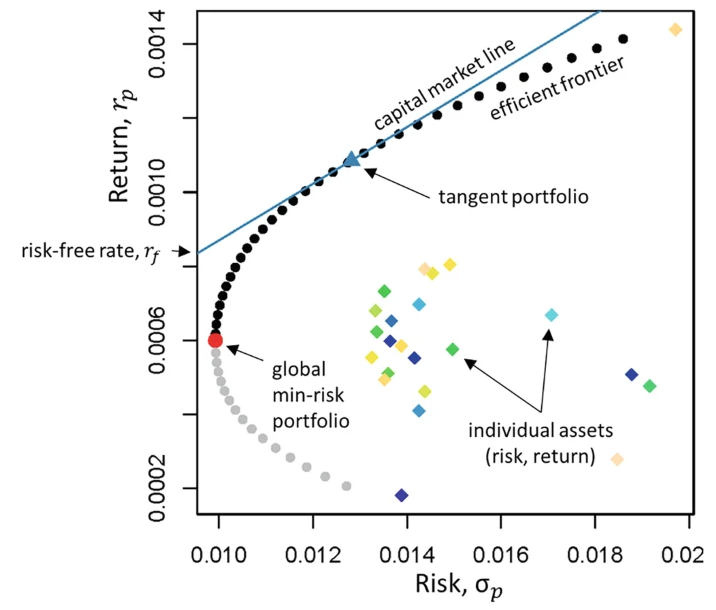
\includegraphics[width=0.65\textwidth]{resources/Bildschirm.png}
    \caption{Example showing the fundamental elements of MPT optimization: Efficient Frontier, global minimum-risk and tangency portfolio. Source: Lindquist, W. B., Rachev, S. T., Hu, Y., \& Shirvani, A. (2022). Modern portfolio theory. In \textit{Advanced REIT portfolio optimization: Innovative tools for risk management} (pp. 29–48). Springer International Publishing.}
    \label{fig:1}
\end{figure}


\subsubsection{The Maximum Sharpe Ratio Portfolio}
The Sharpe ratio is defined as 

\begin{equation} \label{eq: sr}
    SR = \frac{E[\mu - r_f]}{\sigma_p}
\end{equation}

where $\mu$ is the expected return of the portfolio and $r_f$ is the return of the risk-free asset (refer to Section \ref{data} for calculation details). The term in the numerator reflects the portfolio's excess return over the risk-free rate. The term in the denominator represents the standard deviation of the portfolio's excess return over the risk-free rate (\citep{sharpe1994sharpe}). When evaluating two portfolios, the one with a higher Sharpe ratio indicates a more favorable return per unit of risk compared to the one with a lower Sharpe ratio. Thus, the Sharpe ratio quantifies how well the return of a portfolio compensates the risk taken (\citep{gatfaoui2009sharpe}).

The maximum Sharpe ratio portfolio, also known as the tangency or tangent portfolio, represents the optimal portfolio in the presence of a risk-free asset. As can be seen in figure \ref{fig:1}, this portfolio lies at the intersection between the Efficient Frontier curve and the tangent drawn from the risk-free rate (\citep{bodnar2024constructing}).

\subsection{Methodology \label{method}}

Our research is focusing on generating two types of optimal portfolios: minimum variance and maximum Sharpe ratio. Our models are based on the following assumptions:

\begin{itemize}
    \item  Short selling is not allowed 
    \item The weights sum up to 1
    \item The expected return is set at the average daily return of DJIA in October 2019 (refer to Section \ref{data} for more details)
    \item No transaction costs or taxes are considered
    \item The portfolio returns are normally distributed
\end{itemize}


\textbf{Minimum Variance Portfolio}

In a first step, we calculate the minimum variance portfolio (MVP), based on the following formula:

\begin{equation} \label{eq: minvar}
    \min_\omega \omega^T \Sigma \omega \hspace{0.5cm} \text{s.t.} \hspace{0.5cm} 
        \begin{cases} 
            \omega^T \mathbf{r}_T = r_p, \\ 
            \omega^T \mathbf{1} = 1, \\ 
            \omega \geq 0.
        \end{cases} 
\end{equation}

where $\Sigma$ is the the covariance matrix of the asset returns, $\omega$ = $[\omega_1, \omega_2, \dots, \omega_n]$ is the vector comprised of the individual portfolio weights $\omega_i$ and $\mu$ is the target return (refer to Section \ref{data} for calculation details).

In a second step, we calculate the maximum Sharpe ratio portfolio (MSRP).

\textbf{Maximum Sharpe Ratio Portfolio}

The optimization problem in the context of the maximum Sharpe ratio portfolio can be formulated as follows:

\begin{equation} \label{eq: maxsr}
    \max_\omega \frac{\omega^T \mu - r_f}{\sqrt{\omega^T \Sigma \omega}} \hspace{0.5cm} \text{s.t.} \hspace{0.5cm} 
        \begin{cases} 
        \omega^T \mathbf{1} = 1, \\ 
        \omega \geq 0,
        \end{cases} 
\end{equation}

where $\Sigma$ is the covariance matrix of the asset returns, $\omega = [\omega_1, \omega_2, \dots, \omega_n]$ is the vector comprised of the individual portfolio weights $\omega_i$, $\mu$ is a vector of expected portfolio returns, and $r_f$ is the risk-free rate (refer to Section \ref{data} for calculation details).

\textbf{Portfolio performance}

To assess performance of the portfolios, we used the following metrics:

\begin{itemize}
    \item realized portfolio return,
    \item realised portfolio volatility,
    \item realised Sharpe ratio (calculated using formula \ref{eq: sr}).
\end{itemize}

\subsection{Implementation}

The implementation of the study was done using the Python programming language in Jupyter notebook. After installing and importing all the necessary packages, especially yfinance and pandas, in a first step, the historical daily adjusted close prices of the 30 constituents of the DJIA for the research period and the daily yield for the 10-year US Treasury yield were downloaded (chart of the 10-year US Treasury yield can be found in the Appendix \ref{yield}).

In the second step, the log returns and the first 4 moments of the respective returns were calculated (mean, variance, skewnesses and kurtosis). Appendix \ref{moments} contains the results of the calculation for the dataset, along with information on the applicable stock industry. 

We also calculated the correlation matrix of the shares, to ensure the possibility of diversification. Please refer to Appendix \ref{corr}  for a heat-map of the correlations.

To set up the Markowitz optimizations, different variables such as the forecasting period (monthly) and the rebalancing interval (biweekly) were defined. For both the minimum variance and the maximum Sharpe ratio portfolio optimization problems, we used the $cvxopt$-package to optimize equations \ref{eq: minvar}  and \ref{eq: maxsr} using quadratic programming. 

In the next step, the optimization problems were defined subject to constrains given in \ref{eq: minvar} and \ref{eq: maxsr}. We subsequently checked for optimization failures. A rolling window approach was taken to forecast the covariances of the securities and derive optimal weights. 

To evaluate the performance of the portfolios, we  conducted back-testing. The optimal portfolio variances, the portfolio returns and the Sharpe ratios were stored. In addition, we also calculated the performance of an equally weighted portfolio as a benchmark and compared the results of the optimized portfolios to it.

For both the minimum variance and the maximum Sharpe ratio optimizations and also for the equally weighted portfolio, we generated scatter plots that depict the portfolio's return, volatility and Sharpe ratio at each rebalancing step. Finally, we visualized the difference between the optimized portfolios compared to the benchmark portfolio throughout the time period under investigation for the three different performance measures.

\newpage

\section{Results and Empirical Analysis}

\subsection{Descriptive Analysis}
When looking at the evolution of the 10-Year Treasury yield (refer to Appendix \ref{yield} for the chart), we see a large decrease in yield starting with the outbreak of COVID-19 in early spring of 2020. The yield has then remained at a comparatively low level for the rest of the time period under investigation. 

The 4 moments calculation (refer to Appendix \ref{moments} for the table) showed us that most of the shares tend to have slightly negative skewness and relatively high kurtosis, which implies higher risks of negative returns and outliers (heavy tails).

 The visual analysis of the heat map (refer to Appendix \ref{corr} for the figure) shows below-average correlations among stocks. There are several instances with low correlation, which is particularly valuable from a diversification perspective.

\subsection{Portfolio Performance}

\subsubsection{Overall Portfolio Performance}

Following deriving optimal weights we performed back-testing of all the considered models on realized data as mentioned in Section \ref{method}. Figure \ref{fig:scatter} summarizes obtained back-testing results. 

\textbf{Minimum Variance Portfolio}

The scatter plot of the minimum variance portfolio illustrates the objective of the minimum variance portfolio, which is to reduce the volatility. Especially compared to the scatter plot of the maximum Sharpe ratio strategy, we see that most point cluster at a low volatility level. When observing the y-axis, we see that most points are around zero percent return, with some positive and some negative outliers. The Sharpe ratios are also predominantly negative.


\begin{figure}[H]
    \centering
    \begin{minipage}{0.7\textwidth}
    \centering
    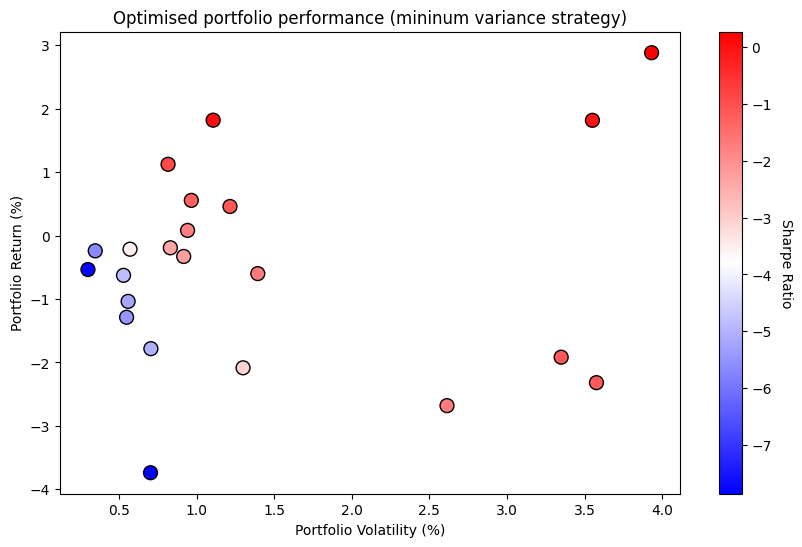
\includegraphics[width=1\textwidth]{resources/Optimised portfolio performance (minimum variance portfolio).png}
    \end{minipage}
    \hfill
    \begin{minipage}{0.7\textwidth}
    \centering
    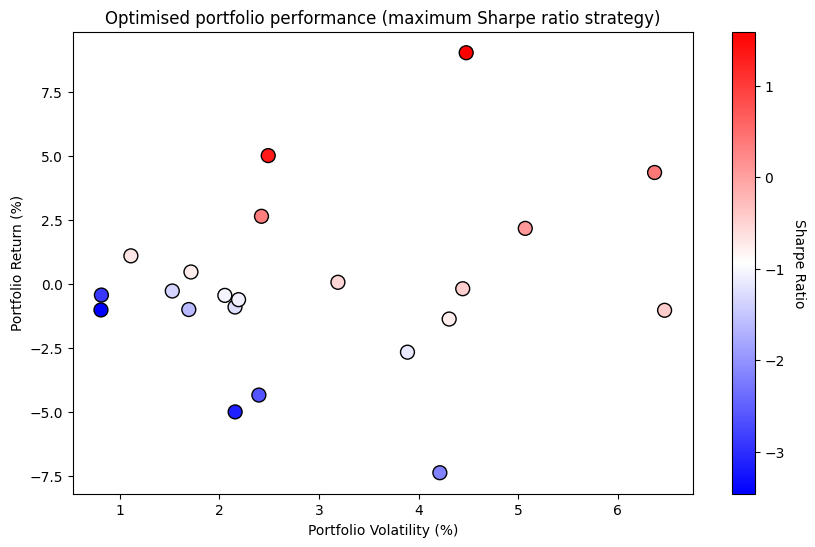
\includegraphics[width=1\textwidth]{resources/Optimised portfolio performance (maximum sharpe ratio strategy).png}
    \end{minipage}
    \begin{minipage}{0.7\textwidth}
    \centering
    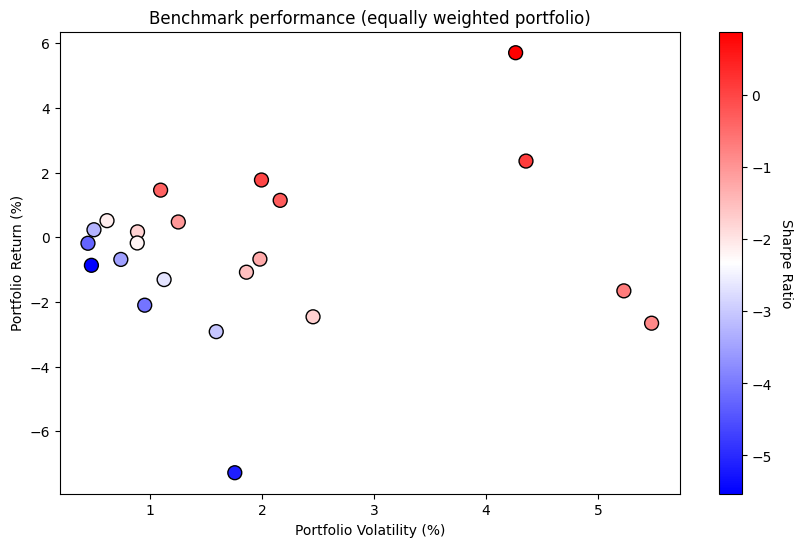
\includegraphics[width=1\textwidth]{resources/Benchmark performance (equally weighted portfolio).png}
    \end{minipage}
    \caption{Portfolio performance back-testing results}
    \label{fig:scatter}
\end{figure}


\textbf{Maximum Sharpe Ratio Portfolio}

For the scatter plot of the MSRP, we can observe that the points in general are more dispersed compared to the scatter plot of the MVP. We have a maximum return of more than 7.5\% in one point and the lowest return is at around -7.5\%. We also observe that here, we have more portfolios with a positive Sharpe ratio compared to the plot of the MVP.

\textbf{Equally Weighted Portfolio}

On the scatter plot of the equally weighted portfolio we also observe a cluster of points around zero percent return, however, it is not as concentrated compared to the MVP. We also observe that the Sharpe ratio of the equally weighted portfolios are predominantly negative, such as in the case of the MVP.


\subsubsection{Comparison to benchmark}

In order to assess whether MVP or MSR portfolios could still benefit investors, we compared results to an equally weighted portfolio (used as a benchmark as mentioned in Section \ref{method}). Figure \ref{fig:compare} provides an overview of the differences between each optimized portfolio performance against the benchmark for all the measures considered in the research: return, volatility and Sharpe ratio. 

\textbf{Volatility}

During the entire period that we have observed, we see that the MVP against the benchmark has always had a lower volatility compared to the MSRP against the benchmark. At the beginning of the COVID-19 crisis in early spring 2020, we can see in both cases that the volatility was less than the one of the benchmark. We can also observe a sharp increase in volatility for the MSRP in the summer months of 2020, while the MVP remains relatively stable.

\begin{figure}[H]
    \centering
    \begin{minipage}{0.7\textwidth}
    \centering
    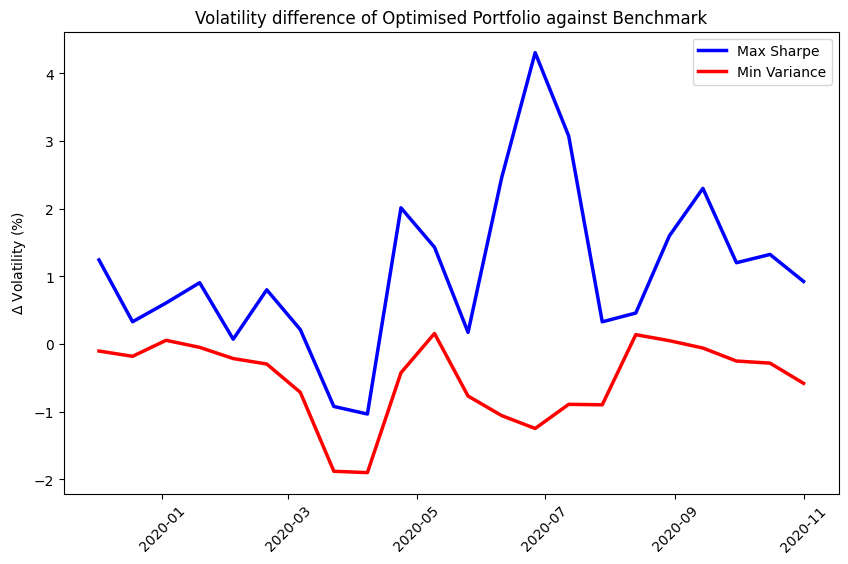
\includegraphics[width=1\textwidth]{resources/Volatility difference of Optimised Portfolio against Benchmark.png}
    \end{minipage}
    \hfill
    \begin{minipage}{0.7\textwidth}
    \centering
    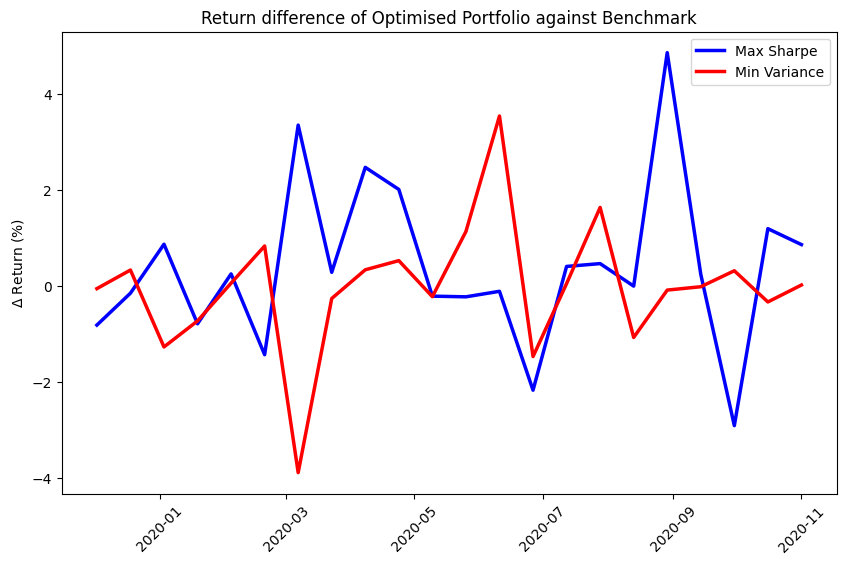
\includegraphics[width=1\textwidth]{resources/Return difference of Optimised Portfolio against Benchmark.png}
    \end{minipage}
    \begin{minipage}{0.7\textwidth}
    \centering
    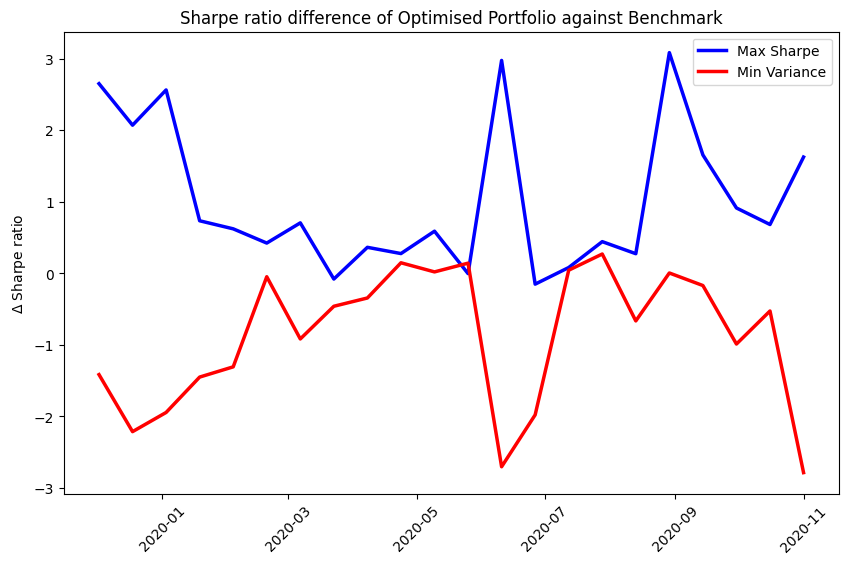
\includegraphics[width=1\textwidth]{resources/Sharpe Ratio.png}
    \end{minipage}
    \caption{Difference of optimsed portfolios against benchmark (equally weighted portfolio)}
    \label{fig:compare}
\end{figure}




\textbf{Return}

At the onset of the COVID-19 crisis, the return of the MVP relative to the benchmark experienced a sharp decline. However, it rebounded quickly, returning to approximately zero. In contrast, the return of the MSRP relative to the benchmark remained positive during this period. During the summer months of 2020, the MVP outperformed the MSRP. By September 2020, the MSRP exhibited significantly higher returns relative to the benchmark compared to the MVP, which remained relatively stable in the subsequent months of the observed period. Toward the end of 2020, between autumn and early winter, the return of the MSRP relative to the benchmark experienced a disctinct decline.


\textbf{Sharpe Ratio}

During the entire period under review, the MSRP against the benchmark almost always had a larger Sharpe ratio compared to the MVP against the benchmark. The Sharpe ratio of the MVP was almost always lower than or equal to the Sharpe ratio of the benchmark. On the other hand, the Sharpe ratio of the MSRP was almost always larger than the one of the benchmark. Before the start of the COVID-19 pandemic, the difference between MSRP and MVP in the context of the Sharpe ratio was large, however, with the start of the crisis, the difference between the two decreased. Between June and Juyl 2020, we observe a distinct increase in Sharpe ratio for the MSRP and also an evident decrease of the MVP. 

\subsection{Key Findings}

The key findings of this research include that the none of the analysed models consistently derived stable positive results when compared using key metrics: return, volatility and the Sharpe ratio. Each model exhibited trade-offs in performance, which further confirms the difficulty in managing portfolio of large-cap stocks in course of market distress.

Maximum Sharpe ratio generated higher returns and Sharpe ratios, however, at the cost of increased risk (i.e. volatility), while minimum variance portfolio achieved on average the lowest volatility, but mostly generating negative returns. Overall, outperforming the benchmark - equally weighted portfolio - proved to be challenging also in course of market turbulence, experienced during the COVID-19 pandemic.

Given our findings, it would be beneficial to further consider alternative hedging instruments to benefit from the diversification results, such as commodity derivatives, Treasury Inflation-Protected Securities, or other financial instruments negatively correlated with blue-chip stocks. Inclusion of such assets may result in improved portfolio performance, especially during market disruptions. 


\newpage
\bibliographystyle{plainnat}
\bibliography{references}

\clearpage

\section{Appendices}
\subsection{Risk free rate overview \label{yield}}
\begin{figure}[htbp]
    \centering
    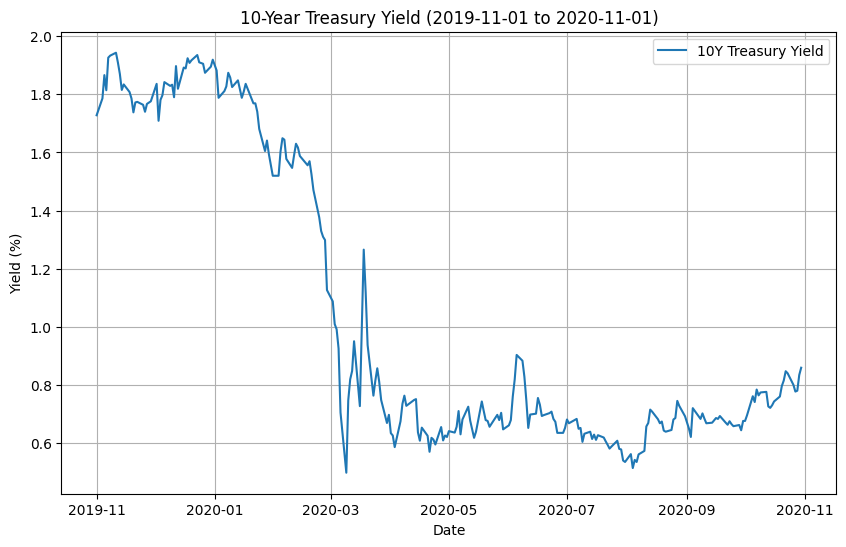
\includegraphics[width=1\textwidth]{resources/10-Year Treasury Yield.png}
\end{figure}
\newpage
\subsection{Four moments overview \label{moments}}
\begin{table}[h!]
\centering
\raggedleft
\renewcommand{\arraystretch}{1} % Adjust row spacing
\setlength{\tabcolsep}{5pt} % Adjust column spacing
\begin{tabular}{|l|r|r|r|r|l|}
\hline
\textbf{Ticker} & \textbf{Mean (\%)} & \textbf{Variance (\%)} & \textbf{Skewness} & \textbf{Kurtosis} & \textbf{Industry} \\ \hline
BA   & -0.35 & 0.29 & -0.32 & 6.21  & Aerospace \& Defense            \\ \hline
RTX  & -0.21 & 0.12 & -0.17 & 5.10  & Aerospace \& Defense            \\ \hline
JPM  & -0.11 & 0.11 & -0.21 & 6.74  & Banks - Diversified             \\ \hline
KO   & -0.05 & 0.05 & -0.77 & 4.14  & Beverages - Non-Alcoholic       \\ \hline
GS   & -0.06 & 0.10 & -0.15 & 6.42  & Capital Markets                 \\ \hline
DOW  & -0.06 & 0.15 & -1.13 & 9.67  & Chemicals                       \\ \hline
CSCO & -0.11 & 0.07 & -0.37 & 6.53  & Comm. Equipment         \\ \hline
MMM  & -0.02 & 0.06 & -0.19 & 4.95  & Conglomerates                   \\ \hline
AAPL & 0.21  & 0.08 & -0.34 & 4.41  & Consumer Electronics            \\ \hline
AXP  & -0.11 & 0.14 & 0.40  & 7.39  & Credit Services                 \\ \hline
V    & 0.00  & 0.07 & -0.14 & 7.46  & Credit Services                 \\ \hline
WMT  & 0.07  & 0.04 & 0.95  & 9.24  & Discount Stores                 \\ \hline
JNJ  & 0.02  & 0.04 & 0.19  & 5.48  & Drug Manf. - General    \\ \hline
MRK  & -0.05 & 0.04 & -0.11 & 4.33  & Drug Manf. - General    \\ \hline
PFE  & -0.03 & 0.04 & -0.25 & 3.95  & Drug Manf. - General    \\ \hline
DIS  & -0.04 & 0.08 & -0.09 & 5.78  & Entrmnt                   \\ \hline
CAT  & 0.03  & 0.08 & -0.81 & 5.03  & Farm \& Heavy Const. \\ \hline
NKE  & 0.12  & 0.07 & -0.19 & 7.83  & Footwear \& Accessories         \\ \hline
UNH  & 0.08  & 0.09 & -0.81 & 9.28  & Healthcare Plans                \\ \hline
HD   & 0.05  & 0.08 & -1.93 & 18.19 & Home Impr. Retail         \\ \hline
PG   & 0.04  & 0.04 & 0.12  & 8.23  & Household \& Personal Prds  \\ \hline
IBM  & -0.08 & 0.07 & -0.51 & 5.60  & IT Services \\ \hline
TRV  & -0.03 & 0.10 & -2.17 & 16.60 & Insurance\\ \hline
CVX  & -0.20 & 0.14 & -1.12 & 14.37 & Oil \& Gas Integrated           \\ \hline
XOM  & -0.30 & 0.10 & -0.21 & 3.27  & Oil \& Gas Integrated           \\ \hline
WBA  & -0.21 & 0.08 & -0.01 & 3.31  & Pharmaceutical Retailers        \\ \hline
MCD  & 0.04  & 0.06 & -0.29 & 18.11 & Restaurants                     \\ \hline
INTC & -0.10 & 0.11 & -0.87 & 11.89 & Semiconductors                  \\ \hline
MSFT & 0.14  & 0.07 & -0.46 & 7.64  & Software - Infra       \\ \hline
VZ   & -0.02 & 0.02 & 0.50  & 5.75  & Telecom Services                \\ \hline
\end{tabular}
\caption{Descriptive statistics of selected companies.}
\label{tab:company_statistics}
\end{table}

\newpage
\subsection{Correlation matrix \label{corr}}
\begin{figure}[h!]
    \centering
    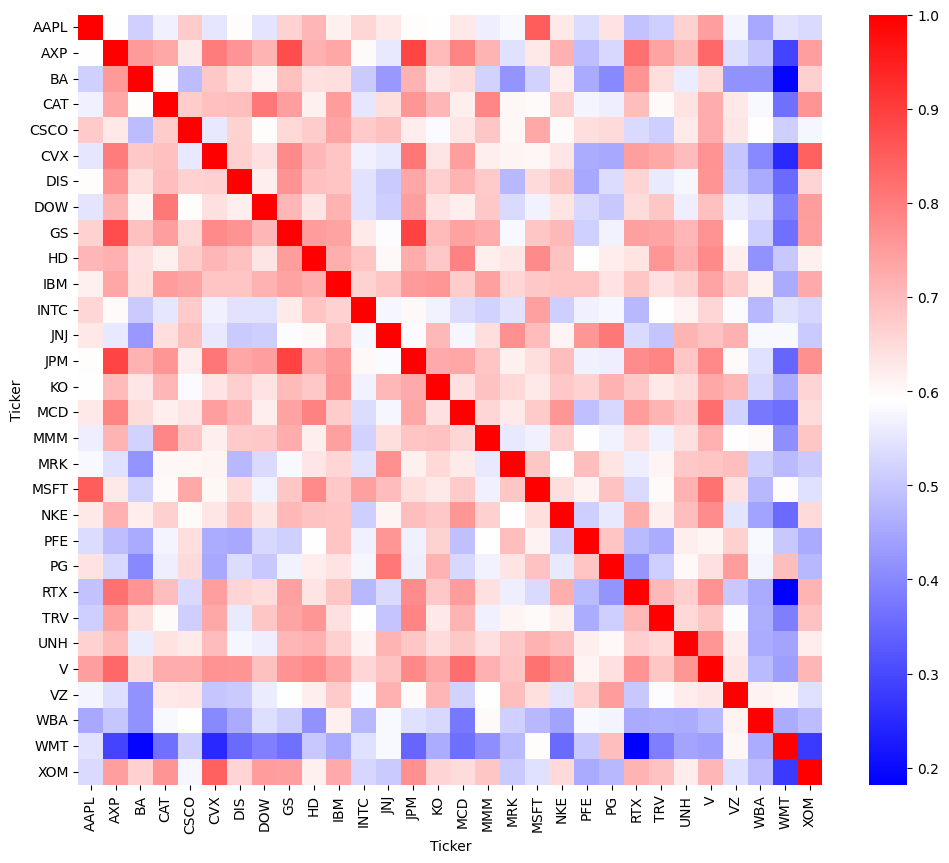
\includegraphics[width=1\textwidth]{resources/Correlation Matrix of DJ constituents.png}
\end{figure}


\end{document}
